\documentclass{beamer}
\usepackage{amsmath,amssymb,amsthm,slashed, euscript}
\usepackage{mathrsfs} 

\usepackage{tikz}
\usepackage{tikz-cd}

%\usepackage{mathtools}

\usetikzlibrary{matrix}
\usetikzlibrary{cd}


\textwidth=110mm


\title{Hurewicz homomorphism of $C^*$-algebras}
\institute
{
 Algebras in analisys
}

\author{Petr R. Ivankov  }



\theoremstyle{plain}
\newtheorem{empt}{}
\newtheorem{defn}{Definition}
\newtheorem{rem}{Remark}
\newtheorem{exm}{Example}
\newtheorem*{claim}{Claim}
\newtheorem{prop}{Proposition}
\newtheorem{lem}{Lemma}%[section]
\newtheorem{thm}{Theorem}%[section]



\newcommand{\A}{\mathcal{A}}
\newcommand{\be}{\begin{equation}}
\newcommand{\ee}{\end{equation}}
\newcommand{\Ga}{\Gamma}
\newcommand{\B}{\mathcal{B}}
\newcommand{\Cc}{\mathcal{C}}
\newcommand{\C}{\mathbb{C}}
\newcommand{\D}{\mathcal{D}}
\newcommand{\G}{\mathcal{G}}
\newcommand{\Hc}{\mathcal{H}}
\newcommand{\Lc}{\mathcal{L}}
\newcommand{\Pc}{\mathcal{P}}
\newcommand{\Sc}{\mathcal{S}}
\newcommand{\U}{\mathcal{U}}
\newcommand{\rar}{\rightarrow}
\newcommand{\Ef}{\mathbb{E}}
\newcommand{\desc}{\mathfrak{desc}}
	\newcommand{\Z}{\mathbb{Z}}                  %% integers
	\newcommand{\Q}{\mathbb{Q}}                  %% rational numbers
	\newcommand{\R}{\mathbb{R}}                  %% rational numbers

	\newcommand{\im}{\mathrm{im}}       %%
	\newcommand{\E}{\mathcal{E}}                 %% space of distributions
	\newcommand{\F}{\mathcal{F}}                 %% space of distributions
	

\newcommand{\ga}{\gamma} 
%Uppercase Gothic characters
\newcommand{\gtA}{\mathfrak{A}}
\newcommand{\gtB}{\mathfrak{B}}
\newcommand{\gtM}{\mathfrak{M}}
\newcommand{\gtN}{\mathfrak{N}}
\newcommand{\gtP}{\mathfrak{P}}
\newcommand{\gtS}{\mathfrak{S}}
\newcommand{\K}{\mathcal{K}}

%Lowercase Gothic characters
\newcommand{\gtf}{\mathfrak{f}}
\newcommand{\gtg}{\mathfrak{g}}
	\newcommand{\End}{\mathrm{End}}       %%

%Bold Characters
\newcommand{\Cb}{\mathbb{C}}
\newcommand{\Nb}{\mathbb{N}}
\newcommand{\Rb}{\mathbb{R}}
\newcommand{\Zb}{\mathbb{Z}}

%Uppercase Greek characters
\newcommand{\Gm}{\Gamma}
\newcommand{\Te}{\Theta}
\newcommand{\Om}{\Omega}
\newcommand{\s}{ }
	\newcommand{\om}{\omega}                     %% short for \omega

%Lowercase Greek characters
\newcommand{\al}{\alpha}
\newcommand{\gm}{\gamma}
\newcommand{\dl}{\delta}
\newcommand{\sg}{\sigma}
\newcommand{\ph}{\varphi}
\newcommand{\te}{\theta}
\newcommand{\ze}{\zeta}
\newcommand{\lift}{\mathfrak{lift}}
\newcommand{\eps}{\varepsilon}                    %% tensor product


\newcommand{\Id}{\mathrm{Id}}
\newcommand{\Aut}{\mathrm{Aut}}
\newcommand{\Coo}{{\mathrm{C}}^\infty}
\newcommand{\alg}{\mathrm{alg}}
\newcommand{\diag}{\mathrm{diag}}
\newcommand{\spinc}{\textbf{$spin^c$}}
\newcommand{\Hom}{\mathrm{Hom}}
\newcommand{\supp}{\mathrm{supp}}
\newcommand{\Ccl}{\mathbf{C}l}
\newcommand{\xto}{\xrightarrow}
\newcommand{\T}{\mathbb{T}} 
\newcommand{\lto}{\longrightarrow}
\newcommand{\ox}{\otimes}
\newcommand{\nb}{\nabla}
\newcommand{\sS}{\mathcal{S}}
\newcommand{\Dn}{D\!\!\!\!/}
%\newcommand{\ij}{{i,j}}
\newcommand{\aC}{\ensuremath{\underline{\Cb}} }
\newcommand{\scp}[2]{\left\langle{#1},{#2}\right\rangle}
\newcommand{\op}[1]{J{#1}J^\dag}
\newcommand{\sA}{\mathcal{A}} 
\newcommand{\sB}{\mathcal{B}}       %%
\newcommand{\sC}{\mathcal{C}}       %%
\newcommand{\sD}{\mathcal{D}}       %%
\newcommand{\sE}{\mathcal{E}}       %%
\newcommand{\sF}{\mathcal{F}}       %%
\newcommand{\sG}{\mathcal{G}}       %%
\newcommand{\sH}{\mathcal{H}}       %%
\newcommand{\sI}{\mathcal{I}}       %%
\newcommand{\sJ}{\mathcal{J}}       %%
\newcommand{\sK}{\mathcal{K}}       %%
\newcommand{\sL}{\mathcal{L}}       %%
\newcommand{\sM}{\mathcal{M}}       %%
\newcommand{\sN}{\mathcal{N}}       %%
\newcommand{\sO}{\mathcal{O}}       %%
\newcommand{\sP}{\mathcal{P}}       %%
\newcommand{\sQ}{\mathcal{Q}}       %%
\newcommand{\sR}{\mathcal{R}}       %%
\newcommand{\sT}{\mathcal{T}}       %%
\newcommand{\sU}{\mathcal{U}}       %%
\newcommand{\sV}{\mathcal{V}}       %%
\newcommand{\sX}{\mathcal{X}}       %%
\newcommand{\sY}{\mathcal{Y}}       %%
\newcommand{\sZ}{\mathcal{Z}}       %%
\newcommand{\N}{\mathbb{N}}                  %% 
	\newcommand{\Ext}{\mathrm{Ext}}       %%
	\renewcommand{\th}{\theta}

\renewcommand{\a}{\alpha}     
\newcommand{\la}{\lambda}     
\newcommand{\La}{\Lambda}
\newcommand{\bt}{\beta}           %% short for  \beta
 \renewcommand{\H}{\mathcal{H}}               %% Hilbert space
 
 	\newcommand{\bean}{\begin{eqnarray*}}
 	\newcommand{\eean}{\end{eqnarray*}}
    
\newcommand{\bydef}{\stackrel{\mathrm{def}}{=}}  
\newcommand{\hookto}{\hookrightarrow}        %% abbreviation
  \usepackage{graphicx}
  \graphicspath{ {./images/} }
  \usepackage{tikz}
\usetikzlibrary{calc,trees,positioning,arrows,chains,shapes.geometric,%
	decorations.pathreplacing,decorations.pathmorphing,shapes,%
	matrix,shapes.symbols}
	
	\usetikzlibrary{trees,positioning,shapes,shadows,arrows}
  

\tikzset{
	basic/.style  = {draw, text width=2cm, drop shadow, font=\sffamily,     rectangle},
	root/.style   = {basic, rounded corners=2pt, thin, align=center,
		fill=green!30},
	level 2/.style = {basic, rounded corners=6pt, thin,align=center,     fill=green!60,
		text width=8em},
	level 3/.style = {basic, thin, align=left, fill=pink!60, text width=6.5em}
}
\begin{document}
%\titlepage
\begin{frame}
  \titlepage
\end{frame}
\begin{frame}
\begin{defn}
	An open connected subset $\sU\subset \sX$ of a topological space is said to be \alert{semilocally proper} if it is evenly covered by any covering $\widetilde{\sX}\to\sX$.
	A space $\sX$ is said to be \alert{weakly semilocally 1-connected} if for  every point $x$ and there is a semilocally proper neighborhood.
\end{defn} 
\end{frame}
\section{$K$-theory and coverings}

	%6.6. 
	Let $p : \sX \to \sY$ be an $n$-fold covering of $\sY$. If $\E$ is a vector bundle over $\sX$, we 
	define a vector bundle $\F = p_*\left( \E\right) $ over $\sY$ by the formula $\F_y \oplus \E_x$. More precisely, if $\sU$ is an open subset in $\sU$ such that $\sV = p^{-1}\left(\sU \right) \cong \sU \times D$ where $D$ is 
	discrete, we give $\F_\sU$ the topology induced by the bijection $\F_\sU \cong \left(\E_\sV \right)^D$.
	\begin{enumerate}
		\item[(a)] Prove that with the topology defined above, $\F$ is a well-defined vector 
		bundle over $\sY$. 
		\item[(b)] Prove that the correspondence $\E \mapsto \F$ induces a group homomorphism 
		$p_*:K\left(\sX \right) \to K\left(\sY \right)$. Moreover, prove the formula 
		$$
		p_*\left(p^*\left(y \right)\cdot x  \right) = y \cdot p_*\left(x \right) 
		$$
		
		for $y\in K\left( \sY\right)$ and $x \in K\left(\sX \right)$,
		\item[(c)]   We assume that $p : \sX \to \sY$ is a \textit{principal} covering with group $G$ (i.e. the finite 	group $G$ acts freely on $\sX$, and $\sY \cong X/G$. Now prove that $p_*\left(p^*\left(y \right)\sum_{g \in G}\rho\left( g\right)^*\right) \left( x\right)$  
		where $\rho\left( g\right)^*K\left(\sX \right)\to K\left(\sX \right)$ is the automorphism of $K\left(\sX \right)$  induced by the action of 	$g$. Prove also that $p_*\left(1 \right)  = \left[\E\right]$ where $\E \bydef \sX \times_G k^n$ $n = \left|G \right|$  and $G$ acts 
		on $k^n$ by the regular representation. 
		
	\end{enumerate} 


\section{Classical Hurewicz homomorphism}
\begin{frame}
	One has the  \alert{Hurewicz homomorphism} 	$h_1:\pi_1\left(\sX, x_0 \right)\to K^1\left(\sX \right)$ such that
	\bean
	\begin{split}
		h^{\mathrm{top}}_{K^1}	:\pi_1\left(\sX, x_0 \right)\cong \left[S^1, s_0; \sX, x_0\right]\xrightarrow{K^1}\\ \Hom\left(K^1\left(C\left( S^1\right)  \right), K^1\left(C\left( \sX \right) \right)\right) \xrightarrow {\phi} K^1\left(C\left( \sX \right) \right).
	\end{split}
	\eean
	Let us describe $h^{\mathrm{top}}_{K^1}$ in details. The map $K^1$ is a functor of $K^1$-homology. 
	If the $C^*$-algebra  $C\left( S^1\right)$ be a $C^*$-algebra generated by a single unitary element $u$, then the group $K^1\left( S^1\right)$  is generated by an element $\left[u\right]$ which is represented by $u$.  $K^1\left( S^1\right)$ is a free Abelian group generated  $\left[ 	K^1_{S^1}\right]$ which corresponds to the identical homomorphism $$\Id_\Z \in \Hom\left( K^1\left(C\left( S^1\right) \cong \Z \left[u\right] \right), \Z \right).$$  
	The Hurewicz homomorphism is given by
	
	\bean
	\begin{split}
		h^{\mathrm{top}}_{K^1}	:\pi_1\left(\sX, x_0 \right)\to K^1\left(C\left( \sX \right) \right),\\
		\left[\om \right] \mapsto K^1\left( \om \right) \left( \left[ 	K^1_{S^1}\right]\right) .
	\end{split}
	\eean
	
	
\end{frame}

\section{Known $C^*$-algebras which admits Hurewicz homomorphism}
\begin{frame}
\centering	\Large	Known $C^*$-algebras  admitting fundamental group\normalsize
	
	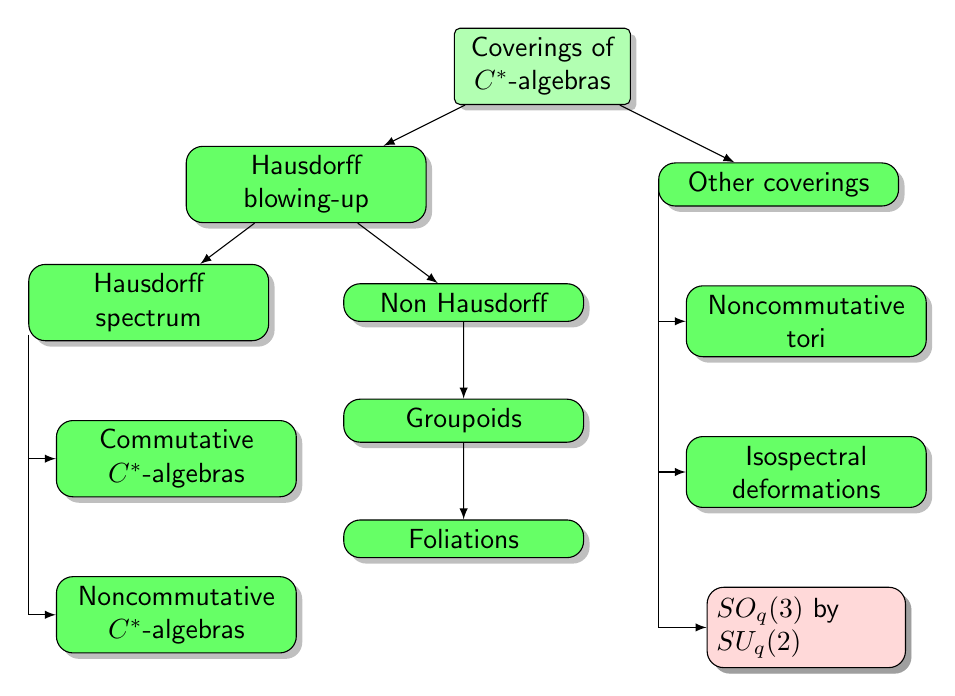
\begin{tikzpicture}[
		level 1/.style={sibling distance=60mm},
		level 2/.append style={sibling distance=40mm},
		edge from parent/.style={->,draw},
		>=latex]
		
		% root of the the initial tree, level 1
		\node[root] {Coverings of $C^*$-algebras}
		% The first level, as children of the initial tree
		child {node[level 2] (ch1) {Hausdorff blowing-up}
			child {node[level 2] (c1) {Hausdorff spectrum}}
			child {node[level 2] (c2) {Non Hausdorff}}{
				child {node[level 2] (c3) {Groupoids}}{
					child {node[level 2] (c4) {Foliations}}
				}
			}
		}
		child {node[level 2] (ch2) {Other coverings}
		};
		\begin{scope}[every node/.style={level 2}]
			\node [below = of  ch2, xshift=10pt] (ch21) {Noncommutative tori};
			\node [below = of  ch21] (ch22) {Isospectral deformations};
			\node [level 3] [below = of  ch22]  (ch23) {$SO_q(3)$ by $SU_q(2)$};
		\end{scope}	
		\begin{scope}[every node/.style={level 2}]
			\node [below = of  c1, xshift=10pt] (c11) {Commutative $C^*$-algebras};
			\node [below = of  c11] (c12) {Noncommutative $C^*$-algebras};
		\end{scope}	
		\foreach \value in {1,...,2}
		\draw[->] (c1.195) |- (c1\value.west);	
		\foreach \value in {1,...,3}
		\draw[->] (ch2.180) |- (ch2\value.west);
	\end{tikzpicture}	
	
\end{frame}
\section{Finite-fold coverings}
\begin{frame}
	\begin{center}
	\huge{Finite-fold coverings}
	\end{center}
	\begin{theorem} 	\alert{Alexander Pavlov, Evgenij Troitsky}.
		Suppose both $\mathcal X$ and $\mathcal Y$ are compact Hausdorff connected spaces and $p :\mathcal  Y \to \mathcal X$
		is a continuous surjection. If $C(\mathcal Y )$ is a projective finitely generated Hilbert module over
		$C(\mathcal X)$ with respect to the action
		\begin{equation*}
			(f\xi)(y) = f(y)\xi(p(y)), ~ f \in  C(\mathcal Y ), ~ \xi \in  C(\mathcal X),
		\end{equation*}
		then $p$ is a finite-fold  covering.
	\end{theorem}
	It is naturally to define a finite-fold covering of $C^*$-algebras as an injective $*$-homomorphisms $A\hookto \widetilde A$ such that $ \widetilde A$-is a finitely generated Hilbert module over
	$A$. However this definition does not gives good generalizations of results  related to topological coverings.
	
\end{frame}
\begin{frame}
  \begin{definition}
	We say that a $C^*$-algebra $A$ is \alert{connected} if it cannot be represented as a direct sum  $A \cong A' \oplus A''$ of nontrivial $C^*$-algebras $A'$ and $A''$.
	
	% (the Gelfand spectrum of the center of $M\left( A\right) $ is connected). Let $A \subset B$ be a connected subalgebra. We say that $A$ is a \alert{connected component} of $B$ if  $1_{M\left( A\right) }$ lies in the center of $1_{M\left( B\right) }$.
\end{definition}
\begin{definition}
	A connected closed two-sided ideal $A$ of  $C^*$-algebra $B$ is said to be a \alert{connected component of}  $B$ is there is a direct sum $B = A \oplus A'$ of $C^*$-algebras.
	\end{definition}
\end{frame}
\begin{frame}
	\begin{definition}\alert{Pet Ivankov}.
		Let $\pi: A \hookto \widetilde{A}$ be an injective *-homomorphism of connected  $C^*$-algebras such that following conditions hold:
		\begin{enumerate}
			\item[(a)] If $\Aut\left(\widetilde{A} \right)$ is a group of *-automorphisms of $\widetilde{A}$ then the group  
			$
			G \bydef \left\{ \left.g \in \Aut\left(\widetilde{A} \right)~\right|~ g\pi\left( a\right)  = \pi\left( a\right) ;~~\forall a \in A\right\}
			$
			is finite.
			\item[(b)] 	\bean
			\pi\left( 	A\right)  = \widetilde{A}^G\stackrel{\text{def}}{=}\left\{\left.a\in \widetilde{A}~~\right|~ a = g a;~ \forall g \in G\right\}.\eean
		\end{enumerate}
		We say that the quadruple $\left(A, \widetilde{A}, G, \pi \right)$ and/or *-homomorphism $\pi: A \to \widetilde{A}$   is a \alert{noncommutative finite-fold  pre-covering}. 
	\end{definition}
	
\end{frame}
\begin{frame}
	\begin{definition}
		\alert{Petr Ivankov}
		Let $\left(A, \widetilde{A}, G, \pi \right)$ be a  noncommutative finite-fold  pre-covering. Suppose both $A$ and  $\widetilde{A}$ are unital. We say that $\left(A, \widetilde{A}, G, \pi \right)$ is an \alert{unital noncommutative finite-fold  covering} if $\widetilde{A}$ is a finitely generated projective  $A$-module.
	\end{definition}
	\begin{lemma}
		\alert{Petr Ivankov, Alexander Pavlov, Evgenij Troitsky.}
		If $\mathcal  X$ is a connected, compact, Hausdorff space then there is a natural 1-1 correspondence 
		$$
		\left(p:\widetilde{\mathcal  X}\to \mathcal  X \right)\leftrightarrow \left(C\left(\mathcal  X\right), C\left(\widetilde\sX\right), G\left(\left.\widetilde{\mathcal  X} \right|\mathcal  X\right), C_0\left(p \right)  \right).  
		$$	
		
		between finite-fold transitive coverings of $\mathcal  X$ and unital noncommutative finite-fold  coverings of $C\left(\mathcal  X\right)$.
	\end{lemma}
	A covering $p:\widetilde\sX\to \mathcal  X $ is \alert{transitive}  if for all $x \in \sX$  the group $G\left(\left.\widetilde{\mathcal  X} \right|\mathcal  X\right)$ transitively acts on $p^{-1}\left( x\right)$. 
\end{frame}

\begin{frame}
	
\begin{definition}
	Let $\left(A, \widetilde{A}, G, \lift \right)$ be a noncommutative finite-fold  pre-covering  of $C^*$-algebras $A$ and $\widetilde{A}$ such  that following conditions hold:
	\begin{enumerate}
		\item[(a)] 
		There are unitizations $A \hookto B$  and $\widetilde{A} \hookto \widetilde{B}$ ;
		%	\item[(b)]$A = B\bigcap \widetilde{A}$,
		\item[(b)] There is a %(strong) 
		unital  noncommutative finite-fold quasi-covering	$\left(B ,\widetilde{B}, G, {\lift}^B \right)$  such that
		$\lift = {\lift}^B|_A$ (or, equivalently $\widetilde A$ is the generated by $A$ hereditary subalgebra of $\widetilde B$) and
		the action $G \times\widetilde{A} \to \widetilde{A}$ comes from  the $G \times\widetilde{B} \to \widetilde{B}$ one.
	\end{enumerate}
	We say that the triple $\left(A, \widetilde{A}, G \right)$ and/or the quadruple $\left(A, \widetilde{A}, G, \lift \right)$ and/or $*$-homomorphism $\lift: A \hookto \widetilde{A}$ is a
	\alert{noncommutative finite-fold covering with unitization}. 
\end{definition}

\end{frame}
\begin{frame}
	Roughly speaking the above  Definition is an approximation of any covering by coverings with compact spaces.	
	In result one has the following theorem.
	\begin{theorem}
		\alert{Petr Ivankov}. 	Let $\mathcal X$ be a connected, locally compact, Hausdorff space.
		If the  quadruple $\left(C_0\left(\mathcal  X \right), \widetilde{A}, G,    \pi\right)$ is a noncommutative finite-fold covering then there is a connected space $\widetilde{   \mathcal X }$ and a transitive finite-fold covering  $p: \widetilde{   \mathcal X } \to \sX$ such that
		$\left(C_0\left(\mathcal  X \right), \widetilde{A}, G,    \pi\right)$ is equivalent to $\left(C_0\left( {   \mathcal X }\right), C_0\left( \widetilde{   \mathcal X }\right), G\left(\left. \widetilde{   \mathcal X } ~\right| {   \mathcal X }\right), \pi\right)$
	\end{theorem}
This Theorem has a Hausdorff blowing-up generalization.
\end{frame}

\section{Infinite coverings}
	\subsection{Basic example}
\begin{frame}
\begin{center}
\huge{Infinite coverings} \normalsize\
\end{center}

	Let $\widetilde \sX$ be a topological space with an action $  G\times \widetilde \sX\to \widetilde\sX$ of residually finite group $  G$  of properly discontinuous  group of homeomorphisms. Let $\sX \bydef \widetilde\sX/   G$ and $p: \widetilde \sX\to\sX$ be a natural covering. 	For any finite factor group $G_\la =  G/ H_\la$ we define a space $\sX_\la \bydef \widetilde \sX/ H_\la$. Then there is a category of topological spaces and finite-fold transitive coverings given by
	\be
	\mathfrak{S}_p \bydef \left\{\left\{\sX_\la\right\}_{\la \in \La}, \left\{p^\mu_\nu:\sX_\mu\to \sX_\nu\right\}_{\substack{\mu,\nu \in \La\\\mu\ge\nu}}\right\}.
	\ee
	Usage of the functor $C_0$  yields a category of $C^*$-algebras and $*$-homomorphisms given by
	\bean
	\begin{split}
		\mathfrak{S}_{C_0\left(p\right) } \bydef \\
		\left\{ \left\{ C_0\left( p_\la\right)  :C_0\left( \mathcal{X}\right)  \hookto C_0\left( \mathcal{X}_\la\right) \right\}, \left\{ C_0\left( p^\mu_\nu\right)  :C_0\left( \mathcal{X}_\mu\right)  \hookto C_0\left( \mathcal{X}_\nu\right) \right\}  \right\}.
	\end{split}
	\eean
\end{frame}
\begin{frame}
	If  $\widehat{G} \bydef \varprojlim_{\la \in \La} G\left(  \left. \sX_\la~\right|\sX \right)$ is an inverse limit of finite groups  then the group  $\widehat{G}$ is profinite. One has $\sX_\la \bydef \widetilde \sX/ \ker\left( G\left(\left. \widetilde\sX~\right|\sX \right)\to G\left(  \left. \sX_\la~\right|\sX \right)\right)$ and there is an inverse limit $\widehat \sX = \varprojlim_{\la \in \La} \sX_\la$ of topological spaces. There is a natural continuous map $\widetilde{\widehat p}: \widetilde \sX  \to \widehat \sX$. If we consider a  {final} {with respect to the family of maps} $\left\{g \circ \widehat p\right\}_{g\in \widehat{G}}$ topology on $\widehat \sX$  then we obtain a topological space $\overline \sX$.
\end{frame}
\begin{frame}

\begin{lemma}
	Under the above hypotheses  the following conditions hold.
	\begin{enumerate}
		\item[(i)] If $\left\{g_\iota G\left(\left. \widetilde\sX~\right|\sX \right)\right\}_{\iota \in I}$   is  a set of all left  cosets of $G\left(\left. \widetilde\sX~\right|\sX \right)$ in $\widehat{G}$  then there is a natural homeomorphism 
		\bean
		\overline \sX \cong \bigsqcup_{\iota\in I} g_\iota \widetilde\sX.
		\eean
		
		\item[(ii)] The natural map $\widetilde{\widehat p}: \widetilde \sX  \to \widehat \sX$ yields a natural inclusion $\widetilde \sX \subset \overline \sX$ such that $\widetilde \sX$ is a quasi-component  of $\overline \sX$.
		\item[(iii)] For any  a quasi-component $\widetilde \sX' \subset \overline \sX$ there is $g \in \widehat{G}$ such that $\widetilde \sX' = g \widetilde \sX$.
		\item[(iv)]  For any $\la \in \La$ the natural surjective map $\widehat p_\la: \widehat \sX \to \sX_\la$ yields a covering  $\overline p_\la: \overline \sX \to \sX_\la$ such that $\sX_\la\cong \overline\sX/ \ker \left(\widehat{G} \to G_\la \right)$. 
		\item[(v)] There is a natural bijective continuous map $\overline{\widehat p}: \overline \sX \to \widehat \sX$.
	\end{enumerate}	
\end{lemma}

\end{frame}
\begin{frame}
	\begin{definition}
		Under the  hypotheses of the above Lemma  we say that the map $\overline p: \overline \sX  \to  \sX$  is the \alert{disconnected covering of} $p : \widetilde \sX \to \sX$. The {topological} $\overline \sX$-$\widehat  G$-{category} $\mathfrak{S}_p$ is the \alert{finite covering category of} $p : \widetilde \sX \to \sX$.
		Write
		\bean
		\mathfrak{S}_p \bydef \left\{\left\{\sX_\la\right\}_{\la \in \La}, \left\{p^\mu_\nu:\sX_\mu\to \sX_\nu\right\}_{\substack{\mu,\nu \in \La\\\mu\ge\nu}}\right\}.
		\eean
		We say that $p : \widetilde \sX \to \sX$ is the \alert{covering inverse limit of} $\mathfrak{S}_p$
		and we write
		\bean
		\widetilde \sX \bydef \varprojlim \mathfrak{S}_p
		\eean
	\end{definition}

\end{frame}
\subsection{General theory}

\begin{frame}
 	If  $\widehat{G}$ is a profinite group   then 
$\widehat{G} \bydef \varprojlim_{\la \in \La}  G_\la$ is an inverse limit of finite groups. The set $\La$ is directed. Indeed $\La$ is the $\widehat{G}$-set. Let $\overline A$ be a $C^*$-algebra with an action $\widehat{G}\times \overline A\to \overline A$ such that any $ g \in \widehat G$ yields an $*$-automorphism of $\overline A$.	  
Suppose that for any element $\overline a \in K\left(\overline A \right)$ of the Pedersen's ideal of $\overline A$  a series 
\bean
\sum_{	g \in \widehat{G}}g \overline a
\eean
is convergent with respect to the strict topology of $M\left(\overline A\right)$.  For any $\la \in \La$ denote by $A_\la$ a generated by elements
\be\label{basic_cov_cl_eqn}
a_\la =\bt\text{-} \sum_{	g \in \ker\left( \widehat{G}\to G_\la\right) }g \overline a
\ee
$C^*$-subalgebra of $M\left(\overline A\right)$, where  $\bt\text{-} \sum$ means a convergence  with respect to the strict topology of $M\left(\overline A\right)$. 
\end{frame}
\begin{frame}
 \begin{lemma}\label{infinite_quasi_covering_lem}
	Under the above hypotheses  all $\mu, \nu \in \La$ such that $\nu\ge\mu$ there is a natural noncommutative finite-fold quasi-covering $\left(A_\mu, A_\la, G_\nu/ G_\mu, \pi^\mu_\nu\right)$.
\end{lemma}
\end{frame}
\begin{frame}
 \begin{definition}\label{infinite_quasicovering_defn} 	Under the above hypotheses    $\la_{\mathrm{min}}\in \La$ is the minimal element and $A\bydef A_{\la_{\min}}$ then we say that the triple $\left( A, \overline A, \widehat G\right)$ is an  \alert{infinite quasi-covering}. We say that $A_\la$ is the $\la$-\alert{descent of} $\overline A$. The natural injective $*$-homomorphism $\lift_\la: A_\la \hookto M\left(\overline A \right)$ is the $\la$-\alert{lift}.
\end{definition}
\begin{definition}\label{infinite_desc_defn}
It is proven that under the above  hypotheses   for all $\la\in\La$ there is a  natural   homomorphism of $A_\la$-$A_\la$-bimodules given by
	\bean
	\begin{split}
		\desc_{\la} : K\left(\overline A \right) \to K\left(A_\la \right),\\
		\overline a \mapsto\bt\text{-} \sum_{	g \in \ker\left( \widehat{G}\to G_\la\right) }g \overline a
	\end{split}
	\eean
	where  $\bt\text{-} \sum$ means the convergence with respect to the strict topology of $M\left(\overline A\right)$. 
	We denote this homomorphism as   $\desc_{\la}$ and we say that it is  the $\la$-\alert{descent}.% If $\la_{\min}\in \La$ is the minimal element (cf. then a given by	
%	$$
%	\desc \bydef \desc_{\la_{\min}}: K\left(\overline A \right) \to K\left(A \right)
%	$$  homomorphism   of $A$-$A$-bimodules is the \alert{minimal descent}.
\end{definition}

\end{frame}


\begin{frame}
 
\begin{definition}
	The  above category is said to be an \alert{algebraical finite covering category} if one has:
	\begin{enumerate}
		\item [(a)] 
		any $\mathfrak{S}$-morphism $\pi^\mu_\nu : A_\mu \hookto A_\nu$ is a noncommutative finite-fold  covering,
		\item[(b)] for all $\la \in \La$ is the $\la$-{descent} $\desc_{\la} : K\left(\overline A \right) \to K\left(A_\la \right)$   is surjective, i.e. $\desc_{\la} \left(  K\left(\overline A \right)\right) = K\left(A_\la \right)$.%, moreover we require that $\desc_{\la} \left(  K\left(\overline A \right)_+\right) = K\left(A_\la \right)_+$. 
	\end{enumerate}
	We write
	\be\label{algebraical_finite_covering_category_eqn}
	\mathfrak{S}\bydef \left\{\left\{A_\la\right\}_{\la\in \La}, \left\{\pi^\mu_\nu : A_\mu \hookto A_\nu\right\}_{\substack{\mu, \nu \in \La\\\mu \le \nu}}\right\}
	\ee
	Moreover the given above infinite quasi-covering $\left( A, \overline A, \widehat G\right)$ is said to be a \alert{pre-covering of the algebraical finite covering category}  $\mathfrak{S}$.
\end{definition}


\end{frame}


\begin{frame}
	It is not clear whether pre-covering of the algebraical finite covering category is always unique. So one needs the following definition.
\begin{definition}
Roughly speaking the  \alert{disconnected infinite noncommutative covering} of $\mathfrak{S}=\left\{\left\{A_\la\right\}_{\la\in \La}, \left\{\pi^\mu_\nu : A_\mu \hookto A_\nu\right\}_{\substack{\mu, \nu \in \La\\\mu \le \nu}}\right\}$ is the union of all pre-coverings.

\end{definition}
\begin{theorem}
	For any algebraical finite covering category
$\mathfrak{S}=\left\{\left\{A_\la\right\}_{\la\in \La}, \left\{\pi^\mu_\nu : A_\mu \hookto A_\nu\right\}_{\substack{\mu, \nu \in \La\\\mu \le \nu}}\right\}$ there is the unique disconnected infinite noncommutative covering.
\end{theorem}
\end{frame}
\begin{frame}
		Let	 $\left(A, \overline{A},\widehat{G} \right)$ be a  disconnected infinite noncommutative covering of $\mathfrak{S}=\left\{\left\{A_\la\right\}_{\la\in \La}, \left\{\pi^\mu_\nu : A_\mu \hookto A_\nu\right\}_{\substack{\mu, \nu \in \La\\\mu \le \nu}}\right\}$. If $\widetilde A$ is a connected component  of $\overline{A}$, i.e. $\overline{A} = \widetilde A \oplus \widetilde A^\perp$, and
	\bean
	G\left(\left.\widetilde{A}~\right| A\right)\bydef 
	\left\{\left. g \in \widehat{G}\right| \forall \widetilde a^\perp \in \widetilde A^\perp \quad g \widetilde a^\perp= \widetilde a^\perp\right\}
	\eean
	then there is a natural action
	\bean
	G\left(\left.\widetilde{A}~\right| A\right)\times \widetilde{A} \to \widetilde{A}.
	\eean
	\begin{definition}
		A  disconnected infinite noncommutative covering 	$\left(A, \overline{A},\widehat{G}\right)$ be of $\mathfrak{S}$  is \alert{good} if  following conditions hold:
		\begin{enumerate}
			\item[(a)] if both $\widetilde{A}'$ and $\widetilde{A}''$ are  {connected components} of $\overline A$ then there is  $g \in \widehat{G}$ such that $g \widetilde{A}'= \widetilde{A}''$,
			\item [(b)] if $\widetilde A$ is a   connected component of $\overline{A}$  then for any $\la \in \La$ the restriction $h_\la|_{\widetilde A}$ is an epimorphism, i. e. $h_\la\left(G\left(\left.\widetilde{A}~\right| A\right) \right) = G\left(\left. A_\la~\right|~A \right)$.
		\end{enumerate}
	\end{definition}

	\end{frame}
\begin{frame}
	\begin{definition}
		If $\left(A, \overline{A},\widehat{G}\right)$ is a good  disconnected infinite noncommutative covering of $\mathfrak{S}=\left\{\left\{A_\la\right\}_{\la\in \La}, \left\{\pi^\mu_\nu : A_\mu \hookto A_\nu\right\}_{\substack{\mu, \nu \in \La\\\mu \le \nu}}\right\}$  then a connected component $\widetilde{A} \subset \overline{A}$ is said to be the \alert{inverse noncommutative limit of} $\mathfrak{S}=\left\{\left\{A_\la\right\}_{\la\in \La}, \left\{\pi^\mu_\nu : A_\mu \hookto A_\nu\right\}_{\substack{\mu, \nu \in \La\\\mu \le \nu}}\right\}$. The  group $G\left(\left.\widetilde{A}~\right| A\right)$  is said to be the \alert{covering transformation group}.  The triple
		\bean
		\left(A, \widetilde{A}, G\left(\left.\widetilde{A}~\right| A\right)\right)
		\eean
		is said to be the  \alert{infinite noncommutative covering} or the  \alert{covering} of  $$\mathfrak{S}=\left\{\left\{A_\la\right\}_{\la\in \La}, \left\{\pi^\mu_\nu : A_\mu \hookto A_\nu\right\}_{\substack{\mu, \nu \in \La\\\mu \le \nu}}\right\}.$$ 
	\end{definition}
	
	\end{frame}
	\begin{frame}
		\section{Applications to commutative $C^*$-algebras}
\begin{theorem}
	If one has 
	\begin{itemize}
		\item the {disconnected  $\overline p: \overline \sX  \to  \sX$ covering of} a covering $p : \widetilde \sX \to \sX$ with connected $\widetilde \sX$ and a residually finite covering group $G\left(\left.\widetilde \sX~\right| \mathcal X\right)$,
		\item the finite covering category 	$\mathfrak{S}_p \bydef \left\{\left\{\sX_\la\right\}_{\la \in \La}, \left\{p^\mu_\nu:\sX_\mu\to \sX_\nu\right\}\right\}$ of $p : \widetilde \sX \to \sX$,
	\end{itemize}
	then  the given by 
	\bean		\begin{split}
		\mathfrak{S}_{C_0\left(p\right) } \bydef \\
		\left\{ \left\{  C_0\left( \mathcal{X}_\la\right) \right\}_{\la\in\La}, \left\{ C_0\left( p^\mu_\nu\right)  :C_0\left( \mathcal{X}_\mu\right)  \hookto C_0\left( \mathcal{X}_\nu\right) \right\}  \right\}
	\end{split}
	\eean	
		
		algebraic finite covering category  is good   and the triple $$\left(C_0\left(\mathcal{X}\right), C_0\left(\widetilde \sX\right) ,G\left(\left.\widetilde \sX~\right| \mathcal X\right)\right)$$ is  the  {infinite noncommutative covering} of $\mathfrak{S}_{C_0\left( p\right) }$.
	
\end{theorem}
There is Hausdorff blowing-up generalization of this theorem.
	\end{frame}
	
\begin{frame}
\begin{definition}
	Let $A$ be a connected $C^*$-algebra, and let 
	$
	\left(A, \widetilde{A}, G\left(\left.\widetilde{A}~\right| A\right)\right)
	$
	be the  {infinite noncommutative covering}  of $$\mathfrak{S}=\left\{\left\{A_\la\right\}_{\la\in \La}, \left\{\lift^\mu_\nu : A_\mu \hookto A_\nu\right\}_{\substack{\mu, \nu \in \La\\\mu \le \nu}}\right\}$$ such that $A = A_{\la_{\mathrm{min}}}$.
	Suppose that $\mathfrak{S}$ contains \alert{all} classes of isomorphisms of  noncommutative finite-fold coverings of $A$. Then the triple $\left(A, \widetilde{A}, G\left(\left.\widetilde{A}~\right|{A}  \right) \right)$ of $\mathfrak{S}$ is said to be the \alert{universal  covering} 
	of $A$.  The group $G\left(\left.\widetilde{A}~\right|{A}  \right)$  is said to be the \alert{fundamental group} of $A$. We use the following notation
	\bean
	\pi_1\left(A \right) \stackrel{\mathrm{def}}{=} G\left(\left.\widetilde{A}~\right|{A} \right).
	\eean
\end{definition}
\end{frame}
\begin{frame}

\begin{definition} 
	Let $P$ be a property of noncommutative finite-fold coverings.	Let $A$ be a $C^*$-algebra, and let 	$	\left(A, \widetilde{A}, G\left(\left.\widetilde{A}~\right| A\right)\right)	$	be the  {infinite noncommutative covering}  of $$\mathfrak{S}=\left\{\left\{A_\la\right\}_{\la\in \La}, \left\{\lift^\mu_\nu : A_\mu \hookto A_\nu\right\}_{\substack{\mu, \nu \in \La\\\mu \le \nu}}\right\}$$ such that $A = A_{\la_{\mathrm{min}}}$.	Suppose that $\mathfrak{S}$ contains \alert{all} classes of isomorphisms of noncommutative finite-fold coverings of $A$  which possess the property $P$. Assume that for all $\mu, \nu \in \La$ such that $\mu \le \nu$ the finite-fold noncommutative cornering  $\lift^\mu_\nu : A_\mu \hookto A_\nu$ possesses the property $P$. 	Then the triple $\left(A, \widetilde{A}, G\left(\left.\widetilde{A}~\right|{A}  \right) \right)$ of $\mathfrak{S}$ is said to be the $P$-\alert{universal  covering} 	of $A$.  The group $G\left(\left.\widetilde{A}~\right|{A}  \right)$  is said to be the $P$-\alert{fundamental group} of $A$. We use the following notation
	\bean
	\pi^P_1\left(A \right) \stackrel{\mathrm{def}}{=} G\left(\left.\widetilde{A}~\right|{A} \right).
	\eean
\end{definition}
\end{frame}
\begin{frame}
\section{Hurewicz homomorphisms for $C^*$-algebras}
Let $P$ be a property of noncommutative finite-fold coverings such that
\bean
\left(A, \widetilde{A}, G\left(\left.\widetilde{A}~\right| A\right)\right)\in P \quad \Leftrightarrow \quad G\left(\left.\widetilde{A}~\right| A\right) \quad \text{is an Abelian group}
\eean
and let $\pi^{\text{ab}}_1\left(A \right)\bydef \pi^{P}_1\left(A \right)$ be the $P$-{fundamental group}. 
There are two homomorphisms
\bean
	h^{\mathrm{free}}_{K^1} : \pi^{\text{ab}}_1\left(A \right)_{\mathrm{free}}\bydef \pi^{\text{ab}}_1\left(A \right)/\pi^{\text{ab}}_1\left(A \right)_{\mathrm{tors}} \to  \Hom\left(  K_1\left( A\right), \Z\right),\\
	h_{K^1}^{\mathrm{tors}} : \pi_1^{\text{ab}}\left(A \right)_{\mathrm{tors}}\to   \mathrm{\Ext}^1\left( K_0(A), \mathbb{Z}\right).
\eean
If $A$ is $N$-algebra then there is an exact sequence 
\begin{equation}\nonumber
	0\to	\mathrm{\Ext}^1\left( K_0(A), \mathbb{Z}\right)  \xrightarrow{\psi} K^1(A) \xrightarrow{\varphi} \mathrm{Hom}(K_1(A), \mathbb{Z}))\to 0.
\end{equation}
Using the above equations we will prove that under some hypothesis ones has:
\begin{enumerate}
	\item If $A$ is a $N$ -algebra then the above invariants  yield the natural homomorphism
	\be\nonumber
	h_{K^1}: \pi^{\text{ab}}_1\left(A \right) \to K^1\left( A\right) 
	\ee
	\item If $A \cong C\left( \sX\right)$ then $	h_{K^1}$ is the topological  Hurewicz homomorphism,
\end{enumerate}
	\end{frame}
\begin{frame}
Let $A$ be an unital $C^*$-algebra with unitary element $u\in A$, and let
\bean
\left(   A , \widetilde A, \Z_n\cong G\left( \left.\widetilde A\right| A\right) ,  \lift \right) 
\eean
be an unital noncommutative finite-fold  covering.  Suppose that there are  $u \in A$ and $v \in \widetilde A$ such that
\bean
\begin{split}
	v^n = u,\\
	\widetilde A\bydef \oplus_{j = 0}^{n-1} \lift \left(A\right)  v^j
\end{split}
\eean
where $\oplus$ means a direct sum of left $A$-modules.
Assume that 
\bean
G\left( \left.\widetilde A\right| A\right) \bydef \left\{ \left.g \in \Aut\left(\widetilde{A} \right)~\right|\forall a \in  \lift\left( A\right)  \quad ga = a\right\} \cong \Z_n,
\\
\forall  m  \in \Z, ~~ \forall \overline k \in 	G\left( \left.\widetilde A\right| A\right)\cong\Z_n,\quad  \forall a \in  \lift\left(  A\right)~~ \overline k \cdot \left(a v^m \right) =  a v^m  e^{\frac{2\pi i m k}{n}}.
\eean
where $k$ is a representative of $\overline k$.
\begin{definition}
	Under the above hypothesis   the  noncommutative finite-fold covering with unitization $\left(   A , \widetilde A, \Z_n\cong G\left( \left.\widetilde A\right| A\right) ,  \lift \right)$ is a \alert{$\left(u, v, n\right)$-covering}.
\end{definition}

\end{frame}
\begin{frame}
	Let $\phi_n$ is a Borel $n^{\mathrm{th}}$ root $\phi_n$ of identity map on the set $\left\{\left. z \in \C\right| \left|z \right|=1\right\}$, i.e.
\bean
\left( \phi_n\right)^n = \Id_{\left\{\left. z \in \C\right| \left|z \right|=1\right\}}
\eean
In particular $\phi_n$ can be given by	
\bean
\phi_n\left( \varphi\right)= e^{\frac{i \varphi}{n}} 
\eean
where $\varphi\in \left(0, 2\pi\right]$ is the angular parameter on $\left\{\left. z \in \C\right| \left|z \right|=1\right\}$.
\end{frame}
\begin{frame}
\begin{defn}
	Let $A$ be a $C^*$-algebra, and let be a property $P_{\mathrm{ab}}$ of noncommutative finite-fold coverings such that
	\bean
	\begin{split}
		\left(A, \widetilde A, G, \lift \right) \in P_{\mathrm{ab}}\quad  \Leftrightarrow G \text{ is an Abelian group}.
	\end{split}
	\eean
	then the $P_{\mathrm{ab}}$-fundamental group of $A$ is the \alert{Abelian fundamental group}. denoted by
	\bean
	\pi_1^{\text{ab}}\left(A \right). 
	\eean
	\end{defn}

\end{frame}
\begin{frame}
	\begin{definition}
		Let $A$ be an unital $C^*$-algebra with a faithful nondegenerate representation $\pi: A \to B\left(\H \right)$. 
		An nontrivial element $x \in K_1\left( A\right)_{\mathrm{free}}\bydef K_1\left( A\right)/K_1\left( A\right)_{\mathrm{tors}}$ is \alert{admissible} if it can be represented by an unitary element $u \in  A$  such that there is a set $\left\{v_{n}\right\}_{n \in \N}\subset B\left(\H \right)\setminus A$ of unital elements with
		\bean
		\begin{split}
			v_n^n=\pi\left(u\right),\\
			\forall n, l \in \N \quad v_{n}^l = v_{nl}. 
		\end{split}
		\eean
		and for any $n \in \N$ there is an $\left( u, v_n, n\right)$-covering.
		$$
		\left(   A , \widetilde A_n, \Z_n\cong G\left( \left.\widetilde A_n\right| A\right) ,  \lift_n \right).
		$$
	\end{definition}

\end{frame}
\begin{frame}
	If $V^{\mathrm{adm}}\subset K_1\left( A\right)_{\mathrm{free}}\otimes \Q$ is a generated by admissible elements subspace then $V^{\mathrm{adm}}$ is isomorphic to  the factor-space of   $K_1\left( A\right)_{\mathrm{free}}\otimes \Q$. Similarly if $K^{\mathrm{adm}}_1\left( A\right)_{\mathrm{free}}\bydef V^{\mathrm{adm}} \cap  K_1\left( A\right)_{\mathrm{free}}$ then $K^{\mathrm{adm}}_1\left( A\right)$ is isomorphic to  a factor-group of a $K_1\left( A\right)_{\mathrm{free}}$. Indeed
\bean
K^{\mathrm{adm}}_1\left( A\right)\cong \Z x_1 \oplus ...\oplus \Z x_p
\eean
where $x_j$ is admissible for any $j \in \left\{1,...,p\right\}$ and there is a (non unique) surjective homomorphism $K_1\left( A\right)_{\mathrm{free}}\to \Z x_j$. Any $x \in \left\{x_1,...,  x_p\right\}$  can be represented by $u \in  A$ satisfying to the above conditions. For any $n \in \N$ let $
\left(A, A_n, \Z_n, \lift_n \right) 
$
For any $n \in \N$ let $
\left(A, A_n, \Z_n, \lift_n \right) 
$
be the required by the above definition unital finite-fold  noncommutative covering.  If $h_{n} : \pi^{\mathrm{ab}}_1\left(A\right)\to \Z_n$ is the natural homomorphism then   any $g \in \pi_1\left(A\right)$ yields a character
\bean
\begin{split}
	\chi^g_n : \Z  x \to \sU\left( 1\right),\\
	k   x \mapsto \frac{h_n\left( g\right) v^k_n}{v_n}= e^{\frac{2\pi i ks}{n}} 
\end{split}
\eean
where  and    $s \in \Z$ is a representative of $h_n\left( g\right)\in \Z_n$. 
\end{frame}
\begin{frame}
Moreover one has
\bean
\forall g_, g_2\in \pi_1\left( A\right)\cong \Z^m\quad \chi^{g_1 + g_2}_n =  \chi^{g_1}_n \chi^{g_2}_n. 
\eean
If $\Q x \bydef \Q \otimes_\Z \Z  x$ then there is a character
\bean
\chi^g_\Q:  \Q x \to \sU\left( 1\right),\\
\forall a \in \Z \quad \forall b \in \N \quad \chi^g_\Q\left(\frac{a}{b} x\right)\bydef \left( \chi^g_b\left( x\right)\right)^a
\eean
such that
\bean
\forall  \frac{a}{b} \in \Z\quad \chi^g_\Q\left( \frac{a}{b} x\right) = 1.
\eean
The map
\bean
\phi^{\mathrm{ab}}_{\left( u_j, v_j, j\right)}: \pi_1\left(A\right)\to \chi\left(\Q x \right),\\
g \mapsto  \chi^g_\Q
\eean
is a homomorphism of groups. 
\end{frame}
\begin{frame}
 For any locally compact Abelian group $G$   one can define its \alert{topological dual} $G^*$ as a group of continuous  characters. For any vector space $V$ over field $K$ there is \alert{algebraic dual} space $V'$ of $K$-linear functionals.
\begin{theorem}
	%THEOREM 3. 
	Let $K$ be a non-discrete locally compact field, and $V$
	a left vector-space of finite dimension $n$ over $K$; let $\chi$ be a non-trivial
	character of the additive group of $K$. Then the topological dual $V^*$ of $V$ is
	a right vector-space of dimension $n$ over $K$; the formula
	$$
	\left\langle v, v^* \right\rangle_V =  \chi\left(\left[v, v'\right] \right) 
	$$
	defines a bijective mapping $v' \mapsto v^*$ of the algebraic dual $V'$ of $V$ onto $V^*$.
	%if x(xy)= I for all x, y in K, this mapping is an isomorphism for thestructures of I/ , V* as right vector-spaces over K.
\end{theorem}

\end{frame}
\begin{frame}
	From the Theorem it turns out that if we consider the  {standard character}
	\bean
	\chi_{\text{standard}}: \R \to \sU\left(1 \right) ,\\
	x \mapsto e^{2\pi i x}
	\eean
	then since $\R$ is a locally compact field any character $\chi : \R \to U\left( 1\right)$ uniquely defines a functional $f_\R : \R \to \R$ with
	$$
	\chi = \chi_{\text{standard}} \circ f_\R.
	$$ 
In particular the explained above character $\chi^q_\Q: \Q x \to U(1)$ is continuous, so it can be uniquely extended up to the character $\chi^q_\R: \R x\bydef \Q x \otimes_\Q \R \to U(1)$.	
There is the unique  functional such 
	$f^g_\R : \R x \to \R$ such that $\chi^g_\R = \chi_{\text{standard}}\circ f^g_\R$. From the our construction   it turns out that $\chi^q_\R\left( \Z\right)= \{1\} $, so $f^\R_g\left( \Z  x \right) \subset \Z$ and the functional $f_\R^g$ yields a homomorphism $\phi_g \in \Hom \left( \Z  x , \Z\right)$.
	

\end{frame}
\begin{frame}
	From the direct sum $K^{\mathrm{adm}}_1\left( A\right)\cong \Z x_1 \oplus ...\oplus \Z x_p$ one can deduce  a non unique  direct sum $K_1\left( A\right)_{\mathrm{free}}\cong \Z x_1 \oplus ...\oplus \Z x_p\oplus K^\perp_1\left( A\right)_{\mathrm{free}}$
Using it  one can construct a homomorphism 
\bean
f^g_x: K_1\left( A\right)_{\mathrm{free}}\to\Z
\eean
and from the above equations it follows that $f^g_x$ linearly depends on $g$, i.e.
\bean
\forall g_, g_2\in \pi^{\mathrm{ab}}_1\left( A\right)\cong \Z^m\quad f^{g_1 + g_2}_x =  f^{g_1}_x+f^{g_2}_x.
\eean 
The formula
$$
f^g = f^g_{x_1} + ... + f^g_{x_p}
$$
yields an element of $\Hom\left(K_1\left( A\right)_{\mathrm{free}}, \Z \right)$.


\end{frame}
\begin{frame}
	In result one has a group homomorphism
	\bean
	\begin{split}
		h^{\mathrm{free}}_{K^1} : \pi_1\left(A \right) \to  \Hom\left(  K_1\left( A\right), \Z\right),\\
		g \mapsto f^g 
	\end{split}
	\eean
\begin{definition}\label{hurewicz_free_defn}
	The homomorphism  $h^{\mathrm{free}}_{K^1}$ is the \alert{free  noncommutative Hurewicz homomorphism}.
\end{definition}
\end{frame}
\begin{frame}
 Let $G$ be a finite Abelian group, and let
\bean 
\left(   A, \widetilde A, G = G\left(\left.\widetilde A \right| A \right)  ,  \lift \right)
\eean
be an unital finite-fold covering. Consider a category of finitely generated projective  $\widetilde A$ - $G$-modules, i.e. $\widetilde A$-modules with equivariant action of $G$. According to the well known result this category Morita equivalent to both:
\begin{itemize}
	\item Category of finitely-generated projective $\widetilde A\rtimes G$-modules where $\widetilde A\rtimes G$ is a crossed product.
		\item Category of finitely-generated projective $A$-modules.
\end{itemize}
So there are natural isomorphisms
\bean
K^{G}_0 \left(\widetilde A \right) \cong K_0 \left(\widetilde A \rtimes G\right) \cong K_0\left(A \right). 
\eean

\end{frame}
\begin{frame}
If $Q$ is a projective finitely generated  $\widetilde A$ - $G$-module  and $Q^G \bydef \left\{q \in Q \left| \forall g \in G\quad gq=q \right.\right\}$ then there is a natural direct sum
$$
Q = Q^G \oplus Q^\perp
$$
since any $q\in Q$ equals to the sum $q^G + q^\perp$ where
\bean
q^G \bydef \frac{1}{\left| G\right| }\sum _{g\in G}g q \in Q^G,\\
q^\perp \bydef q - q^G \in P^\perp.
\eean
Similarly if $r: G \to U\left( 1\right)$ is an irreducible representation then $Q^\perp = Q_r \oplus Q_r^\perp$ since any $p\in P^\perp$ equals to the sum $q_r + q_r^\perp$ where
\bean
q_r\bydef \frac{1}{\left| \ker r\right| }\sum _{g\in \ker r}g q\\
q_r^\perp \bydef q - q_r
\eean

\end{frame}
\begin{frame}
It follows that any projective finitely generated  $\widetilde A$-$G$-module $Q$ is represented by direct sum 
$$
Q = Q^G \bigoplus \left(\bigoplus_{r \in R} Q_r\right) 
$$
where $R$ is a set of irreducible representations of $G$. It turns out that
\bean
K^{G}_0 \left(\widetilde A \right)= \left(K^{G}_0 \left(\widetilde A \right) \right) ^G \bigoplus \left(\bigoplus_{r \in R} K^{G}_0 \left(\widetilde A \right)_r\right)
\eean
For any $r\in R$ there is a prime number $p_r \in \N$ such that $\im ~r = e^{\frac{2\pi i \Z}{p_r}}$. There is $g\in G$ with
\bean
r\left( g\right) =  e^{\frac{2\pi i}{p_r}},\\
\forall r' \in R\setminus \{r\}\quad r'(g)= 1.
\eean

\end{frame}
\begin{frame}
	If $x_1, x_2 \in K^{G}_0 \left(\widetilde A \right)_r$ are such that $\chi_{x_1} \left(g \right) = \chi_{x_2} \left(g \right)= e^{\frac{2\pi i k}{p_r}}$  with $k\in \N$  then one has
	$$
	\forall g \in G \quad\chi_{x_1-x_2} \left(g \right)=\{1\}\quad x_1-x_2 \in  \left(K^{G}_0 \left(\widetilde A \right) \right) ^G
	$$ 
	it is possible if and only if $x_1 - x_2 = 0$. From our construction there is an isomorphism
	$$
	\phi_r : \Z_{p_r} \cong K^{G}_0 \left(\widetilde A \right)_r
	$$
	such that
	$$
	\forall \overline k \in \Z_{p_r} \quad \chi_{\phi_r\left( \overline k\right) }\left( g\right) = e^{\frac{2\pi i k}{p_r}}
	$$
	where $k \in \Z$ is a representative of $\overline{k}$. Moreover any $g \in G$  yield a character
	\be\label{chi_r_eqn}
	\chi_r : K^{G}_0 \left(\widetilde A \right)_r \to U(1).
	\ee
	
Following Lemma is a consequence of the above construction and the isomorphism .

\end{frame}
\begin{frame}
\begin{lemma}\label{h_tors_lem}
	If $R$ is a set of irreducible representations of $G$ then there is a decomposition
	\bean
	K_0\left( A\right) = K_0\left(A \right)^\perp \bigoplus  \left(\bigoplus_{r \in R} K_0 \left( A \right)_r\right).
	\eean
	If $\im ~r = e^{\frac{2\pi i \Z}{p_r}}$ then  $K_0 \left( A \right)_r$ is trivial, or there is an isomorphism $K_0 \left( A \right)_r\cong \Z_{p^r}$.
\end{lemma}


\end{frame}
\begin{frame}
The decomposition of the lemma yield a map from $G$ to the set of characters of  $K_0\left(A \right)$ 
$$
g \mapsto \left(x^\perp + \sum_{r \in \R} x_r \mapsto \prod_{r\in R}\chi_r\left(x_r \right)   \right) 
$$
From 
\bean
\forall g', g'' \in G\quad \chi_{r}\left(g' \right)\chi_{r}\left(g'' \right)= \chi_{P_j}\left(g 'g''\right).
\eean
Using it one can construct  a homomorphism 
\bean
h_{K^1}^{\mathrm{tors}} : G \to   \Ext^1_\Z\left( K_0\left( A\right), \Z \right)
\eean
If $A$ belongs to class $N$  then one has a homomorphism
$$
h_{K^1}^{\mathrm{tors}} : G\to   K^1\left(A \right) 
$$


\begin{definition}\label{hurewicz_torsion_defn}
	The above
	map is the \alert{torsion  of noncommutative Hurewicz homomorphism}.  
	\end{definition}
\end{frame}
\begin{frame}
\begin{definition}\label{hurewicz_admits_defn}
	An unital $C^*$-algebra  $A$ \alert{admits  Hurewicz homomorphism} if one has:
	\begin{enumerate}
		\item[(a)] All Abelian groups $\pi^{\mathrm{ab}}_1\left( A\right)$, $K_0\left( A\right)$ and $K_1\left( A\right)$ are finitely generated.
		\item[(b)] If $\pi^{\mathrm{ab}}_1\left( A\right)_{\mathrm{tors}}\subset \pi^{\mathrm{ab}}_1\left( A\right)$ is the torsion subgroup then there  an unital finite-fold noncommutative covering $\left(   A, \widetilde A,  G\left(\left.\widetilde A \right| A \right)  ,  \lift \right)$ such that the composition $\pi^{\mathrm{ab}}_1\left( A\right)_{\mathrm{tors}} \hookto  \pi_1\left( A\right) \to G\left(\left.\widetilde A \right| A \right)$ is isomorphism.
	\end{enumerate}
\end{definition}
	If an  unital $C^*$-algebra  $A$ {admits  Hurewicz homomorphism} then  $\pi^{\mathrm{ab}}_1\left(A\right)$ is the direct sum of groups
	\be\label{h_dir_prod_eqn}
	\begin{split}
		\pi^{\mathrm{ab}}_1\left( A\right)\cong \pi^{\mathrm{ab}}_1\left( A\right)_{\mathrm{tors}}\oplus
		\pi^{\mathrm{ab}}_1\left( A\right)/\pi^{\mathrm{ab}}_1\left( A\right)_{\mathrm{tors}} \cong\\ G\left(\left.\widetilde A \right| A \right) \oplus \pi_1^{\mathrm{ab}}\left(\widetilde A \right)\cong \\ \cong \pi^{\mathrm{ab}}_1\left( A\right)_{\mathrm{tors}}\oplus
		\pi^{\mathrm{ab}}_1\left( A\right)_{\mathrm{free}}. 
\end{split}
\ee
\end{frame}
\begin{frame}
There   are the free  and the torsion  Hurewicz homomorphisms
\bean
h_{K^1}^{\mathrm{free}} : \pi^{\mathrm{ab}}_1\left( \widetilde A\right) \to \Hom\left( K_1\left( \widetilde A\right) , \Z\right),\\
h_{K^1}^{\mathrm{tors}} : G\left(\left.\widetilde A \right| A \right)\cong \pi^{\mathrm{ab}}_1\left( A\right)_{\mathrm{tors}} \to   \Ext^1_\Z\left( K_0\left( \widetilde A, \Z\right)\right).
\eean
The inclusion  yields a homomorphism $\iota :K_0\left( A\right) \to K_0\left(\widetilde A\right)$ so there are homomorphisms 
\bean
r_1 : \Hom\left(K_1\left(\widetilde A\right), \Z \right) \to \Hom\left(K_1\left(A\right), \Z \right),\\
r_2 : \Ext^1_\Z\left(K_0\left(\widetilde A\right), \Z \right) \to \Ext^1_\Z\left(K_0\left(A\right), \Z \right), \\
\eean 
On the other hand there are subjective homomorphism $s_1 : \pi^{\mathrm{ab}}_1\left(A \right) \to  G\left(\left.\widetilde A \right| A \right)=\pi^{\mathrm{ab}}_1\left( A\right)_{\mathrm{tors}}$ and $s_2 : \pi^{\mathrm{ab}}_1\left(A \right) \to \pi^{\mathrm{ab}}_1\left(\widetilde A \right)$.

\end{frame}
\begin{frame}
\begin{definition}\label{hurewicz_pair_defn}
	If $A$ \alert{admits  Hurewicz homomorphism}  then a pair of  homomorphisms
	\be
	\begin{split}
		h^1_{K^1}\bydef r_1 \circ s_1: \pi^{\mathrm{ab}}_1\left(A \right)\to  \Hom\left(K_1\left(A\right), \Z\right), \\
		h^2_{K^1}\bydef r_2 \circ s_2:\pi^{\mathrm{ab}}_1\left(A \right)\to  \Ext^1_\Z\left(K_0\left(A\right), \Z\right) 
	\end{split}
	\ee
	is the \alert{Hurewicz pair}.
\end{definition}

\end{frame}
\begin{definition}
If $A$ is an $N$-algebra then both direct sum and  exact sequence yield the following diagram
\newline
\begin{tikzcd}
	\pi^{\mathrm{ab}}_1\left( A\right)_{\mathrm{tors}}\arrow[r]\arrow[d, "h^1_{K^1}"]& \pi^{\mathrm{ab}}_1\left( A\right)_{\mathrm{tors}}\oplus
	\pi^{\mathrm{ab}}_1\left( A\right)_{\mathrm{free}}\arrow[r]\arrow[d, "h^A_{K^1}	\bydef h^1_{K^1} + h^2_{K^1}"]& 
	\pi^{\mathrm{ab}}_1\left( A\right)_{\mathrm{free}}\arrow[d, "h^2_{K^1}"]\\
	\mathrm{\Ext}^1\left( K_0(A), \mathbb{Z}\right)\arrow[r, "\psi"]  & K^1(A)\arrow[r, "\varphi"]  & \mathrm{Hom}(K_1(A), \mathbb{Z})).
\end{tikzcd}
So there is the  \alert{unital Hurewicz homomorphism} given by
\bean
h^A_{K^1}	\bydef h^1_{K^1} + h^2_{K^1}:\pi^{\mathrm{ab}}_1\left(A\right)\to  K^1\left(A \right). 
\eean	
\end{definition}
\section{ Hurewicz homomorphism for commutative $C^*$-algebras}
\begin{frame}
\huge  Hurewicz homomorphism for commutative $C^*$-algebras \normalsize

If $\widetilde \sX\to \sX$ is an universal covering  then the Hurewicz homomorphism looks like
$$
h^{C\left( \sX\right) }_{K^1}:G\left(\left.\widetilde \sX \right| \sX\right)\to K^1\left( C\left(\sX \right) \right) 
$$
If $\widetilde \sX$ is not path connected then it is possible that $\pi_1\left(\sX, x_0 \right)$ is trivial but $G\left(\left.\widetilde \sX \right| \sX\right)$ is not trivial the Hurewicz homomorphism of $C^*$-algebras is more informative. 
There is the \alert{weak fundamental group} $\pi^{\mathrm{w}}_1\left(\sX, x_0 \right)$ such that $\pi^{\mathrm{w}}_1\left(\sX, x_0 \right)\cong \pi_1\left(\sX, x_0 \right)$ is $\sX$ is path connected a semilocally 1-connected. However it is possible that $\pi_1\left(\sX, x_0 \right)$ is trivial but  $\pi^{\mathrm{w}}_1\left(\sX, x_0 \right)$ is not trivial. Moreover for any Abelian group $A$ one can define a Hurewicz homomorphism 
\bean
\pi^{\mathrm{w}}_1\left(\sX, x_0 \right)\to \check H_1\left( \sX, A\right)
\eean
to \v{C}ech homology. Above homomorphism have new early unknown type. There are examples nontrivial homomorphisms with trivial  $\pi_1\left(\sX, x_0 \right)$.
 \end{frame}
\begin{frame}
	Let $\sX$ be a compact, connected topological space such that:
	\begin{itemize}
		\item The groups $\pi^{\mathrm{ab}}_1\left(\sX, x_0 \right) $, $K_0\left( C\left(\sX \right) \right)\cong K^0\left(\sX \right) $ and $K_1\left( C\left(\sX \right) \right)\cong K^1\left(\sX \right) )$   are finitely generated Abelian groups,
		\item There is the universal covering $p: \widetilde \sX \to \sX$ with the natural isomorphism $\pi_1\left(\sX, x_0 \right) \cong G\left( \left. \widetilde\sX\right| \sX\right)$. 
	\end{itemize}
	The  (classical) Hurewicz homomorphism $h^{\text{sing}} : \pi_1\left(\sX, x_0 \right)\to H_1\left(\sX \right)$ into singular homology  is an isomorphism. 
	If $\om : \left(S^1, s_0 \right)\to \left( \sX, x_0\right)$ represents an element    $\left[\om\right] \in \pi_1\left(\sX, x_0 \right)$ is  such that
	\bean
	\pi_1\left(\sX, x_0 \right) = \Z \left[\om\right] \oplus  \pi_1\left(\sX, x_0 \right)^\perp.
	\eean
	There is  a surjective homomorphism $\phi_H : H_1\left( \sX\right)\to \Z$ with $\phi_H\left(\Z y \right) = \Z$ and $\phi_H\left(H_1\left( \sX\right)^\perp\right) = \{0\}$. This homomorphism yields an element $z \in H^1\left( \sX, \Z\right)$ with $H^1\left( \sX, \Z\right)=\Z z\oplus  H^1\left( \sX, \Z\right)^\perp$. There is a representative $\varphi_z: \sX \to K\left(\Z, n \right) = S^1$ of $z$.     The composition $\varphi_z \circ \om : S^1 \to S^1$ yields an isomorphism of cohomology of $S^1$ so it is a homotopy equivalence. It follows that there is a surjective homomorphism
	$$
	\pi_1\left(\varphi_z \right) : \pi_1\left(\sX, x_0 \right)\to \pi_1\left(S^1, s_0 \right)\cong \Z.
	$$
	\end{frame}
	\begin{frame}
			\begin{center}
			\centering
			{
				\centering	\Large	Free case\normalsize		}
		\end{center}
	For any $n \in \N$ thee is a there are a finite index subgroup, topological space and two transitive coverings given by 
	\be\label{h_finite_cov_eqn}
	\begin{split}
		H_n \bydef \pi^{-1}_1\left(\varphi_z \right) \left( n \pi_1\left(S^1, s_0\right)  \right)\\
		\widetilde \sX_n  \bydef \widetilde \sX/ H_n,\\
		\widetilde p_n : \widetilde \sX \to \widetilde \sX_n,\\
		p_n : \widetilde \sX_n \to \sX.
	\end{split}
	\ee
	Since $S^1 \cong U\left(1 \right)$ the map $\varphi_z$ yields an unitary element $u \in U\left(C\left( \sX\right)  \right)$.  If  $\pi: C\left( \sX\right)\to B\left(\H_a\right)$ be an atomic representation  and   $\phi_n$ is given is defined above then for any $n > 1$ there is a generally  discontinuous map $v_n \bydef \phi_n \circ \varphi_z: \sX \to U\left( 1\right)\cong S^1 $ which can be regarded as an element of $ B\left(\H_a\right)$. If $v_n$ is continuous map then $v_n$ represents an element $z_n \in H^1\left( \sX, \Z\right)$ with $n z_n = z$. It is impossible since $x$ is not divisible, so $v_n \notin C\left( 
	\sX\right)$. It follows that 
	\bean
	\begin{split}
		v_n^n=\pi\left(u\right),\\
		\forall n, l \in \N \quad v_{n}^l = v_{nl}. 
	\end{split}
	\eean
\end{frame}
\begin{frame}
	If $\widetilde A_n$ is a $C^*$-subalgebra of $B\left(\H_a \right)$  generated by the union $C\left( \sX\right) \cup \{v_n\}$ then $\widetilde A$ is a subalgebra of maps from $\sX \to \C$, so it is commutative, so from the Theorem Gelfand theorem it turns out that  $\widetilde A_n \cong C\left(\widetilde \sX'_n  \right)$. 
	Moreover \be\label{h_fin_x_sum_eqn}
	\begin{split}
		v^n = u,\\
		C\left(\widetilde \sX'_n  \right)= \oplus_{j = 0}^{n-1} \pi \left(C\left(\sX \right) \right)  v^j
	\end{split}
	\ee
	where $\oplus$ means a direct sum of left $A$-modules, i.e. there is an $\left( u, v_n, n\right)$-covering 
	$$
	\left(   C\left( \sX\right)  , C\left(  \widetilde \sX'_n\right) , \Z_n\cong G\left( \left.C\left(  \widetilde \sX'_n\right)\right| C\left(   \sX\right)\right) ,  C\left( p'_n\right)  \right)
	$$
	where $p'_n : \widetilde \sX'_n\to \sX$ is a covering induced by an inclusion $C\left(   \sX\right)\hookto C\left(  \widetilde \sX'_n\right)$.
	\end{frame}
	\begin{frame}
		From $v^n = u$ it turns out that
		$$
	\pi_1\left( \varphi_z \circ p'_n \right) \left(\pi_1\left( \widetilde \sX'_n\right)  \right) = n \pi_1\left( \sX, x_0\right)= \pi_1\left( \varphi_z \circ p_n \right) \left(\pi_1\left( \widetilde \sX_n\right)  \right)
	$$
	and from the above equation it follows that the covering  $p'_n : \widetilde \sX'_n\to \sX$ is equivalent to the  $p_n : \widetilde \sX_n\to \sX$ one.  If $u$ represents a nonzero element $\left[u\right]\in K_1\left(C\left( \sX  \right)\right) $ then   from the above equations  it turns out that $\left[u\right]$ is admissible. For any $n \in \N$ the specialization of the character explained in general theory character
	\bean
	\begin{split}
		\chi^{\left[\om\right]}_n : \Z \left[u\right]\to \sU\left( 1\right),\\
		k   \left[u\right] \mapsto  e^{\frac{2\pi i k}{n}}. 
	\end{split}
	\eean 
	and from the above equation it follows that the covering  $p'_n : \widetilde \sX'_n\to \sX$ is equivalent to the  $p_n : \widetilde \sX_n\to \sX$ one. \label{key}
	Clearly a set $\left\{v_n\right\}_{n \in \N}$ satisfies to the conditions  of the definition of admissible element, i.e. $u$ is admissible.
\end{frame}
\begin{frame}
	  Here we drop analogs manipulations below the equation and   obtain a specialization 
	\bean
	f^{\left[\om\right]}_{\left[u\right]}: K_1\left( A\right)_{\mathrm{free}}\to\Z
	\eean
	of the given by the equation  free Hurewicz homomorphism, i,e. $h_{K^1}^{\mathrm{free}}$ maps $\om$ onto the image of $f^{\left[\om\right]}_{\left[u\right]}$ Using this fact one can prove that free part of classical  free Hurewicz homomorphism coincides with noncommutative one,
 \end{frame}
\section{Torsion case}
\begin{frame}
	\begin{center}
		\centering
		{
\centering	\Large	Torsion case\normalsize		}
	\end{center}
%\centering	\Large	Torsion case\normalsize\\
Let $p \in \N$ be a prime number and $\sX$ is path connected and $\om : \left( S^1, s_0\right)  \to \left(\sX, x_0 \right)$ is a representative of an element $\left[\om \right]\in \pi_1\left(\sX, x_0 \right)$ with  $p\left[\om \right]= 0$. Suppose that there is a $p$-listed  covering $\th_p: \widetilde \sX \to \sX$ such that the composition
$$
\Z\left[\om\right] \cong \Z_p \to \pi_1\left(\sX, x_0 \right) \to G\left(\left. \widetilde \sX \right| \sX \right)
$$
is isomorphism of Abelian groups. It turns out that  the composition $\om \circ \th_p$ represents a trivial element $\left[\om \circ \th_p\right]= p\left[\om \right]\in \pi_1\left(\sX, x_0 \right)$. So there is a homotopy $\Phi : S^1 \times \left[0, 1\right]\to \sX$ with
\bean
\forall s \in S^1 \quad \Phi\left( s, 0\right) = \om \circ \th_p\left( s\right); \\ \Phi\left( s, 1\right) = x_0, \\
\forall t\in  \left[0, 1\right]\quad   \Phi\left(x_0, t\right) = x_0
\eean 
\end{frame}
\begin{frame}
	Let
	$ C'\om$ be the mapping cone defined by the following way:
	\begin{itemize}
		\item there is a mapping cylinder $M_{\th_p}$ (cf. Definition \ref{mapping_cylinder_defn}),
		\item   $C'\om\bydef M_{\th_p} / j\left(S^1 \right)$. 
	\end{itemize}
then  map $\Phi$ yields a composition
$$
S^1  \to C'\om \to \sX.
$$
If $m_0$ corresponds to a base point  of $ C'\om$ then there is a decomposition
$$
S^1   \to C'\om\setminus \{m_0\} \to \sX.
$$
It follows that one has
$$
K^1\left(C\left( S^1\right)  \right) \to K^1\left(C\left( C'\om\setminus \{m_0\}\right)  \right) \to K^1\left(C\left( \sX\right)  \right) 
$$
On the other hand $(C\left( C'\om\setminus \{m_0\}\right)$ is the mapping cone $C_{ C\left(\th_p \right)}$ of the homomorphism $C\left( \th_p\right) : C\left( S^1\right) \hookto C\left(S^1 \right)$. There is a following exact sequence
\bean
0 \to SC\left(S^1 \right) \xrightarrow{\iota} C_{ C\left(\th_p \right)} \xrightarrow{P} C\left(S^1 \right) \to 0.
\eean
	\end{frame}
	\begin{frame}
		From the Puppe sequences 
		\small
\bean
KK\left(SC\left(S^1 \right), SC\left(S^1 \right)  \right)\xrightarrow{KK\left( \Id_{SC\left(S^1 \right)},SC\left(\th_p \right)  \right)} KK\left(SC\left(S^1 \right), SC\left(S^1 \right)  \right)\\\xrightarrow{KK\left( \Id_{SC\left(S^1 \right)},\iota  \right)} KK\left(SC\left(S^1 \right),C\left(C_{\th_p} \right) \right)\xrightarrow{KK\left( \Id_{SC\left(S^1 \right)},P \right)} KK\left(SC\left(S^1 \right), C\left(S^1 \right)  \right) \\ \xrightarrow{KK\left( \Id_{SC\left(S^1 \right)},C\left(\th_p \right)  \right)} KK\left(SC\left(S^1 \right), C\left(S^1 \right)  \right);\\
KK\left(C\left(S^1 \right),C\left(S^1 \right)   \right)\xrightarrow{KK\left(C\left(\th_p \right),\Id_{C\left(S^1 \right) }   \right)} KK\left(C\left(S^1 \right),C\left(S^1 \right)   \right) \xrightarrow{KK\left(P,\Id_{C\left(S^1 \right) }   \right)}\\\to KK\left(C_\phi,C\left(S^1 \right)   \right) \xrightarrow{KK\left(\iota,\Id_{C\left(S^1 \right) }   \right)} KK\left(SC\left(S^1 \right), C\left(S^1 \right) \right)\\\xrightarrow{KK\left(SC\left(\th_p \right),\Id_{C\left(S^1 \right) }   \right)}KK\left(SC\left(S^1 \right),C\left(S^1 \right)  \right).
\eean		\end{frame}
\begin{frame}
\normalsize it follows that	\small
\bean
K_0\left( SC\left(S^1 \right)  \right)\xrightarrow{K_0\left( SC\left(\th_p \right)  \right)} 	K_0\left( SC\left(S^1 \right) \right) \xrightarrow{K_0\left( \iota \right) }  K_0\left(C\left(C_{\th_p} \right) \right)\xrightarrow{K_0\left( p \right)}  	K_0\left( C\left(S^1 \right)  \right) \\ \xrightarrow{K_0\left( C\left(\th_p \right)  \right)} 	K_0\left( C\left(S^1 \right) \right),\\
K^1\left( C\left(S^1 \right)  \right)\xrightarrow{K^1\left( C\left(\th_p \right)  \right)} 	K^1\left( C\left(S^1 \right) \right) \xrightarrow{K^1\left( \iota \right) }  K^1\left(C\left(C_{\th_p} \right) \right)\xrightarrow{K^1\left( p \right)}  	K^1\left( SC\left(S^1 \right)  \right) \\ \xrightarrow{K^1\left( SC\left(\th_p \right)  \right)} 	K^1\left( SC\left(S^1 \right) \right),
\eean
\normalsize So one has
\bean
K_0\left(C\left(C_{\th_p} \right) \right) \cong K^1\left(C\left(C_{\th_p} \right)\right)  \cong \Z_p.
\eean 
\end{frame}


\begin{frame}
\normalsize
The decomposition 
$$
S^1   \to C'\om\setminus \{m_0\} \to \sX
$$
yields the following homomorphisms
$$
K^1\left(C\left(S^1 \right)  \right) \to K\left(C_0\left( C'\om\setminus \{m_0\} \right)  \right) \to K^1\left(C\left(\sX \right)  \right) 
$$
Using the above homomorphisms one can prove the coincidence of classical and noncommutative Hurewicz homomorphism.

\end{frame}
\end{document}























